%% LyX 2.1.4 created this file.  For more info, see http://www.lyx.org/.
%% Do not edit unless you really know what you are doing.
\documentclass[english]{article}
\usepackage[T1]{fontenc}
\usepackage[utf8]{luainputenc}
\usepackage{array}
\usepackage{graphicx}

\makeatletter

%%%%%%%%%%%%%%%%%%%%%%%%%%%%%% LyX specific LaTeX commands.
%% Because html converters don't know tabularnewline
\providecommand{\tabularnewline}{\\}

%%%%%%%%%%%%%%%%%%%%%%%%%%%%%% User specified LaTeX commands.
\usepackage{babel}
\graphicspath{{images/}}


\makeatother

\usepackage{babel}
\begin{document}

\section{One }


\section{Two}


\section{Specific Requirements}

This section of the document is dedicated at giving an in-depth description
of the platform's requirements, and is to be kept as reference during
all future phases of development. 


\subsection{External interfaces}

Being MyTaxiService a fully service-oriented platform, its only external
interfaces must be those reserved for the final users; there is no
need to design specific maintenance access to the back-end system
as this is already fully standardized and does not need specific functionalities
other than the usual system administration tools.

As briefly described in section \ref{sub:User-interface}, the main
principle that must guide the design of the external interfaces of
the platform is that of business identity continuity. This section
contains a set of design mock-ups that are to be kept as reference
during the development of the user interfaces. 


\subsection{Functions}


\subsection{Use Cases}

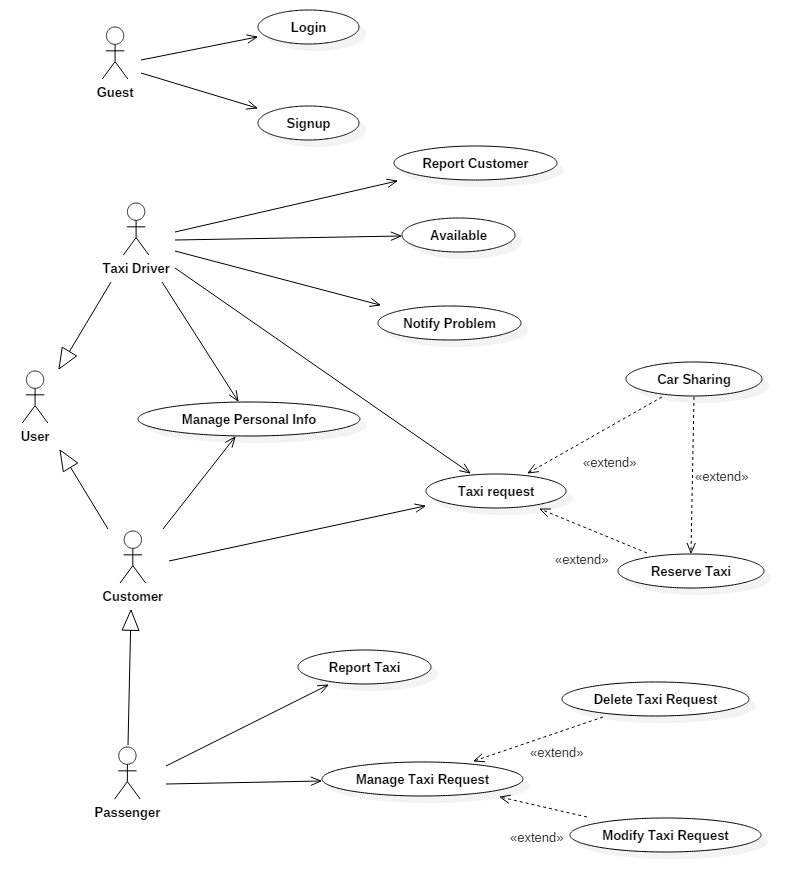
\includegraphics[width=1\textwidth,bb = 0 0 200 100, draft, type=eps]{UseCase}


\subsection{Scenarios}

To help the reader understand the above stated requirements, a brief
description of how a use case might look like in the real world is
given below. 

In the examples, Adam and Joanne are customers who intend to request
a taxi and Hector, Monica, Jim and Samuel are taxi drivers of the
town. 


\subsubsection{Sign up}

Adam has just downloaded the customer-side app and wants to sign up
into the platform. He requests the customer registration page, fills
the form and submit the request to the system. If Adam's e-mail and
username are unique the system gives Adam a confirmation of the success
of the operation and redirects Adam to the login page, otherwise it
displays an error message.


\subsubsection{Login}

Adam, now registered, inserts the username and password in the login
form and clicks the login button; the system checks the information
and, if the username-pasword combination is correct, redirects Adam
to his own user profile page; otherwise, an error message is shown. 


\subsubsection{Available}

Hector, already logged into the platform, starts his working by day
opening his taxi driver profile page and communicating his availability
to the system. The system updates the taxi queue in Hector's zone
and sends Hector a notification with his position in the queue. 


\subsubsection{Taxi request}

Adam, now logged into the system, wants to book a taxi to go home.
He opens the taxi request page on the app, and requests a taxi. The
system forwards Adam's request to the queue associated with Adam's
position, and Hector, which is the first taxi driver in the queue,
is notified with the request. 

Unfortunately, Hector has now decided to take a break and does not
want to take this ride; he refuses Adam's request by tapping a button
on the app, and the system forwards the request to Monica, the taxi
driver immediately after Hector in the queue. 

As she accepts Adam's request, Adam receives a notification on the
app with the estimated waiting time. 


\subsubsection{Book a Taxi}

While on Monica's taxi, Adam wants to book a taxi for that evening
at 6 PM, in order to go to the cinema. He opens the taxi request page
of the app, and fills and submits the request form. 

The system checks the information (sending eventual error notifications
back to Adam) and forwards Adam's request to Jim, by using a specific
selection algorithm over taxi drivers in the queue associated to Adam's
zone. 

Jim decides to accept Adam's booking, and will keep his schedule free
for the time that Adam requested. 


\subsubsection{Manage Taxi Request}

Later that day, Adam opens the ``Manage taxi request'' page from
his laptop's browser to change the booking time from 6PM to 7PM. The
system checks whether Adam's request is feasible (there must be at
least two hours between the current time and the requested time),
and eventually forwards the changes to Jim. 

Jim accepts the modification and a confirmation is sent back to Adam. 


\subsubsection{Report Taxi}

Jim picks Adam up at 7PM. During the ride Jim lights up a cigarette
and is unreasonably rude towards Adam.

Adam opens the ``Report taxi'' page on the app, to file a complaint
about Jim's behavior. The system updates Jim's profile information
with the new report and confirms the success of the operation to Adam.


\subsubsection{Report User}

After the ride, Adam is annoyed by the behavior of Jim and refuses
to pay for the ride. 

Jim opens the ``Report user'' page, fills the complaint form and
submits it to the system. The system updates Adam's profile information
with the new report and confirms the success of the operation to Jim.


\subsubsection{Manage Personal Information}

Joanne has opened a new main email account. 

She opens his profile page from the app, clicks on the edit button
and changes his email address to match the new one; she then submits
the new information. 

The system performs a check on the information, updates Joanne's profile
and notifies the success of the operation to Joanne.


\subsubsection{Report Problem}

During a ride, Hector has a problem with his taxi's engine and can't
bring Joanne to destination. 

Through the ``Report problem'' page of the app, he notifies the
problem to the system, by filling the form and submitting. The system
acknowledges the report and asks Hector if needs a new taxi; Hector
confirms, and the system forwards his request to Samuel, who is the
first taxi driver in Hector and Joanne's current zone. 


\subsection{Flows of events}


\subsubsection{Sign-up}

\begin{tabular}{lp{8cm}}
\hline 
Actors  & Guest \tabularnewline
\hline 
Preconditions  & The guest is not registered into the system \tabularnewline
\hline 
Execution Flow  & \begin{enumerate}
\item The guest requests the registration page 
\item The system asks for the sign-up information 
\item The guest fills the form and submits the request 
\item The system checks the uniqueness of the username and e-mail 
\item The system creates the customer (or taxi driver) profile 
\item The system sends the confirmation to the guest \end{enumerate}
\tabularnewline
\hline 
Postconditions  & The guest is now a registered user \tabularnewline
\hline 
Exceptions  & The e-mail or username are not unique or, in the case of taxi driver
sign-up, the license is not valid \tabularnewline
\end{tabular}

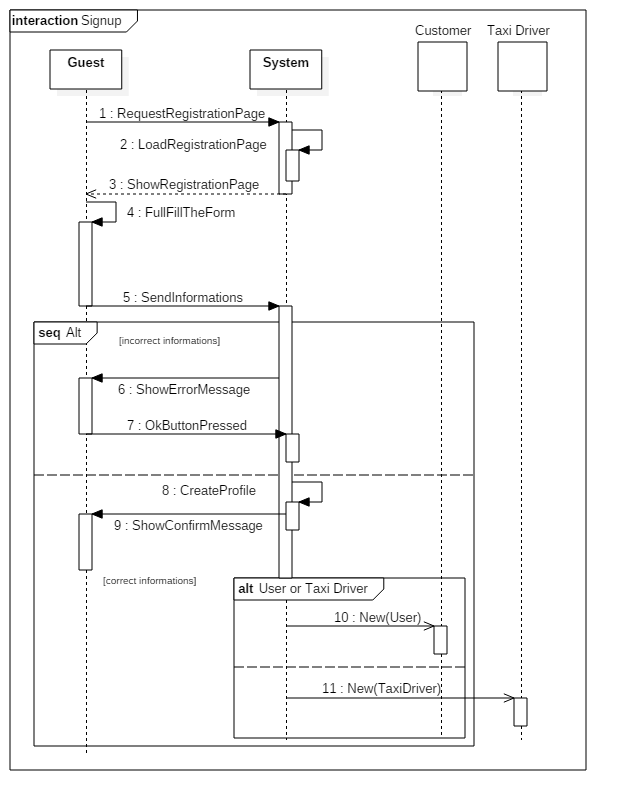
\includegraphics[width=1\textwidth,bb = 0 0 200 100, draft, type=eps]{Signup}


\subsubsection{Login}

\begin{tabular}{lp{8cm}}
\hline 
Actors  & Guest \tabularnewline
\hline 
Preconditions  & The guest has already a profile into the system\tabularnewline
\hline 
Execution Flow  & \begin{enumerate}
\item The guest requests the login page 
\item The system requires the login information (Username, password) 
\item The guest fills the form and submits the request 
\item The system checks the username and password 
\item The system sends a login confirmation 
\item The guest is logged into the system 
\item The guest is redirected to the user profile page \end{enumerate}
\tabularnewline
\hline 
Postconditions  & The guest is now a logged-in user\tabularnewline
\hline 
Exceptions  & The username, password combination is incorrect, so the guest cannot
log in \tabularnewline
\end{tabular}

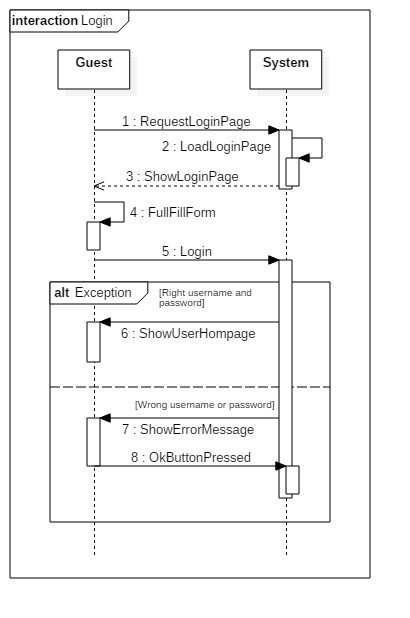
\includegraphics[width=1\textwidth,bb = 0 0 200 100, draft, type=eps]{Login}


\subsubsection{Available}

\begin{tabular}{lp{8cm}}
\hline 
Actors  & Taxi driver \tabularnewline
\hline 
Preconditions  & \tabularnewline
\hline 
Execution Flow  & \begin{enumerate}
\item The taxi driver requests the taxi profile page 
\item The system returns the personal information of the user
\item The taxi driver notifies their availability to the system 
\item The system updates the local queue 
\item The system confirms the request to the taxi driver \end{enumerate}
\tabularnewline
\hline 
Postconditions  & The taxi driver is now available \tabularnewline
\hline 
Exceptions  & \begin{itemize}
\item The taxi driver is located in a invalid zone 
\item The taxi driver is carrying a passenger 
\item The taxi driver is not available\end{itemize}
\tabularnewline
\end{tabular}

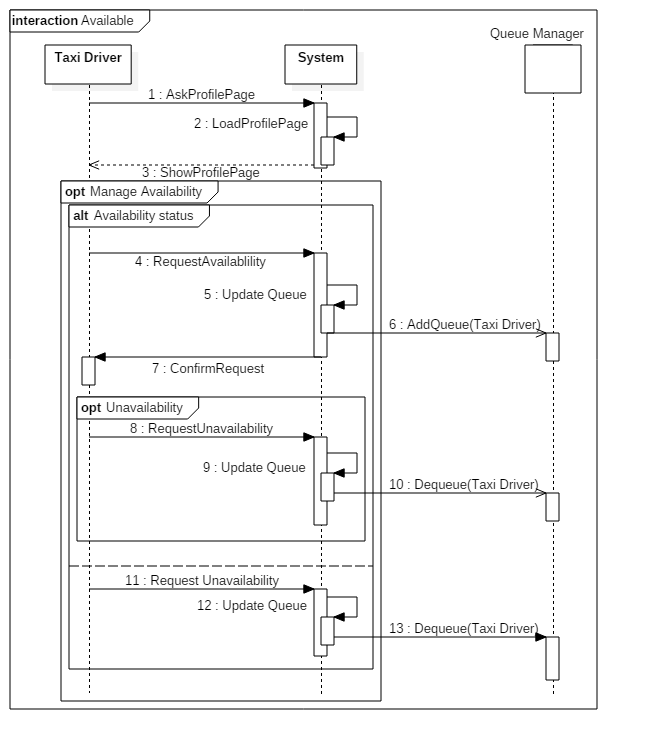
\includegraphics[width=1\textwidth,bb = 0 0 200 100, draft, type=eps]{Available}


\subsubsection{Taxi Request}

\begin{tabular}{lp{8cm}}
\hline 
Actors  & User, Taxi driver \tabularnewline
\hline 
Preconditions  & The user should not be banned \tabularnewline
\hline 
Execution Flow  & \begin{enumerate}
\item The user requests the taxi request page 
\item The system asks for the type of request that the user wants to issue 
\item The user fills the request form and sends the information to the system 
\item The system forwards the request to the first taxi driver of the local
queue 
\item If the taxi driver answers positively to the request, he takes the
user in charge, otherwise he denies the request 
\item If the taxi driver accepts the request, the system notifies to the
user the incoming taxi and changes the availability of the taxi driver;
otherwise, the system updates the queue and forwards the request to
the new first taxi driver of the queue.
\item If there are no taxis available, the system notifies the user.\end{enumerate}
\tabularnewline
\hline 
Postconditions  & If the request is accepted by a taxi driver, the user is now a passenger \tabularnewline
\hline 
Exceptions  & \begin{itemize}
\item The user provides incorrect information in the request form 
\item The user is not in a valid position (\emph{e.g. outside the town}) \end{itemize}
\tabularnewline
\end{tabular}

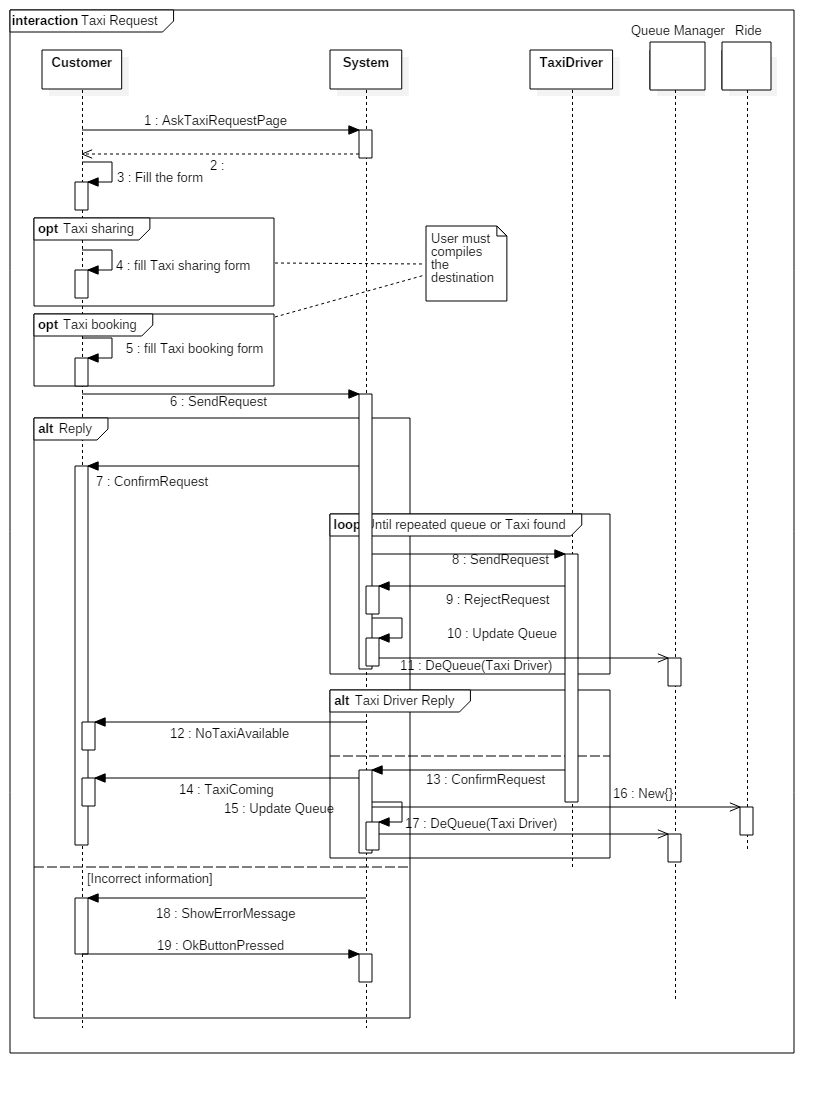
\includegraphics[width=1\textwidth,bb = 0 0 200 100, draft, type=eps]{TaxiRequest}


\subsubsection{Manage Taxi Request}

\begin{tabular}{lp{8cm}}
\hline 
Actors  & Passenger \tabularnewline
\hline 
Preconditions  & \tabularnewline
\hline 
Execution Flow  & \begin{enumerate}
\item The passenger request the taxi Request Management page 
\item The system load the page and return it to the passenger 
\item The passenger can modify the Request full filling the modify Request 
\item The system modify the request and return a confirm to the passenger 
\item The passenger can delete the request, submitting the operation to
the system 
\item The system update the queue and return a confirmation to the passenger \end{enumerate}
\tabularnewline
\hline 
Postconditions  & \begin{itemize}
\item If the passenger choose to modify the Request, the request is updated 
\item If the passenger choose to delete the Request, the request is canceled
and the taxi is now in queue \end{itemize}
\tabularnewline
\hline 
Exceptions  & \begin{itemize}
\item The passenger provides incorrect information in the modify request
form 
\item The passenger cancel the request too late \end{itemize}
\tabularnewline
\end{tabular}

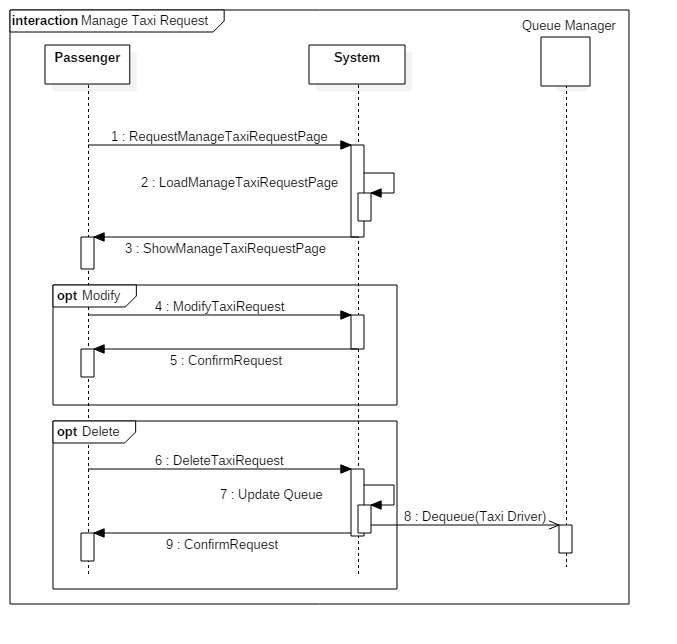
\includegraphics[width=1\textwidth,bb = 0 0 200 100, draft, type=eps]{ManageTaxiRequest}


\subsubsection{Report Taxi}

\begin{tabular}{lp{8cm}}
\hline 
Actors  & Passenger \tabularnewline
\hline 
Preconditions  & \tabularnewline
\hline 
Execution Flow  & \begin{enumerate}
\item The passenger request the Report taxi page 
\item The system elaborate the request and ask to the passenger the report
information 
\item The passenger fill the form and submit the report 
\item The system check the data obtained 
\item The system update the taxi driver information 
\item The system notify to the passenger the successful of the operation \end{enumerate}
\tabularnewline
\hline 
Postconditions  & The taxi driver is reported by the current passenger \tabularnewline
\hline 
Exceptions  & The passenger provides wrong information in the report form \tabularnewline
\end{tabular}

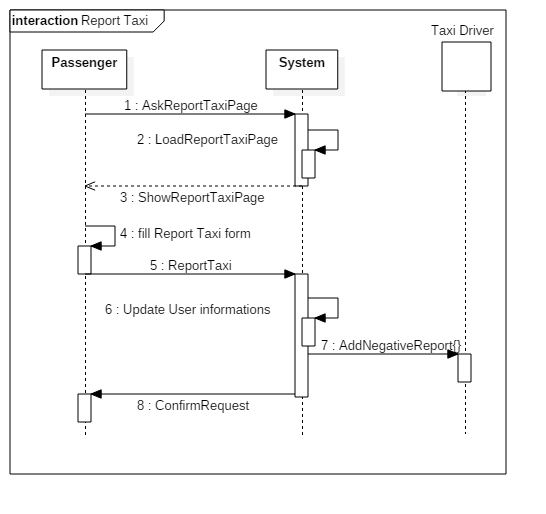
\includegraphics[width=1\textwidth,bb = 0 0 200 100, draft, type=eps]{ReportTaxi}


\subsubsection{Report User}

\begin{tabular}{lp{8cm}}
\hline 
Actors  & Taxi driver \tabularnewline
\hline 
Preconditions  & The taxi driver should had carried the user past 24 hours \tabularnewline
\hline 
Execution Flow  & \begin{enumerate}
\item The taxi driver request the Report user page 
\item The system elaborate the request and ask to the taxi driver the report
information 
\item The taxi driver fill the form and submit the report 
\item The system check the data obtained 
\item The system update the user information 
\item The system notify to the taxi driver the successful of the operation \end{enumerate}
\tabularnewline
\hline 
Postconditions  & The user is reported by the taxi driver \tabularnewline
\hline 
Exceptions  & The taxi driver provides wrong information in the report form \tabularnewline
\end{tabular}

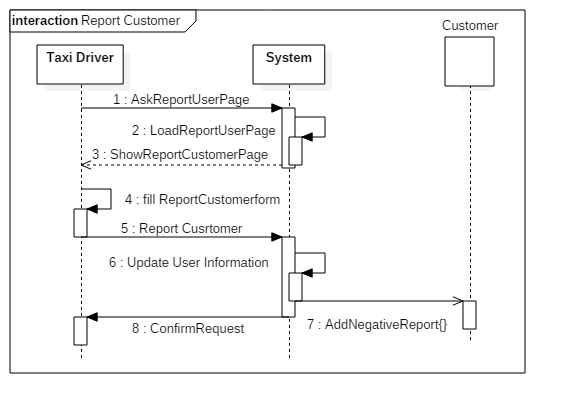
\includegraphics[width=1\textwidth,bb = 0 0 200 100, draft, type=eps]{ReportUser}


\subsubsection{Manage Personal Information}

\begin{tabular}{lp{8cm}}
\hline 
Actors  & User or Taxi driver \tabularnewline
\hline 
Preconditions  & \tabularnewline
\hline 
Execution Flow  & \begin{enumerate}
\item The user (or taxi driver) request the user profile page 
\item The system returns the personal information of the user (or taxi driver) 
\item The user (or taxi driver) can request the edit of the profile 
\item The system return the editable information of the profile 
\item The user (or taxi driver) can edit those data and send the changes
to the system 
\item The system check the correctness of the new information
\item If the information are correct send the Change Confirm to the user
(or taxi driver), otherwise send back an error message \end{enumerate}
\tabularnewline
\hline 
Postconditions  & If the user request a modify profile and submit correct information
the Profile is changed \tabularnewline
\hline 
Exceptions  & The user provides wrong information \tabularnewline
\end{tabular}

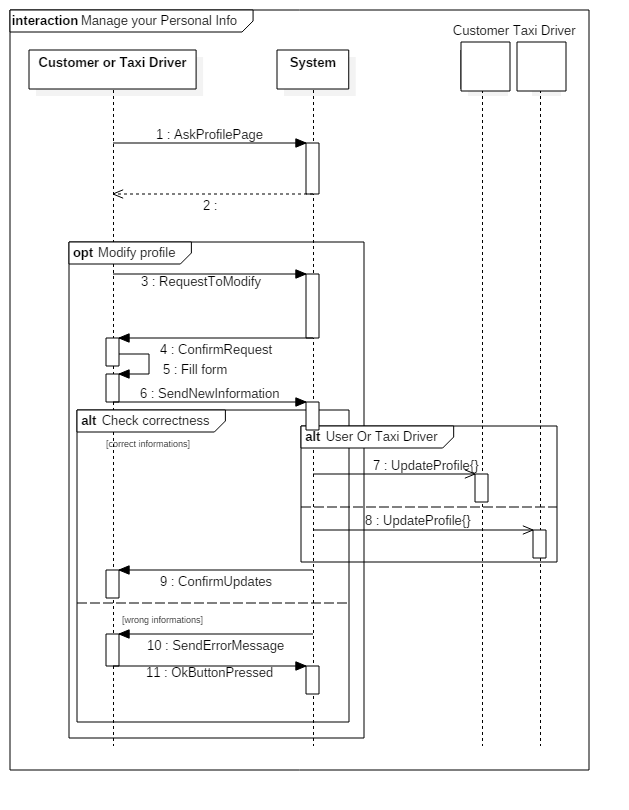
\includegraphics[width=1\textwidth,bb = 0 0 200 100, draft, type=eps]{ManageInformation}


\subsubsection{Report Problem}

\begin{tabular}{lp{8cm}}
\hline 
Actors  & Taxi driver \tabularnewline
\hline 
Preconditions  & \tabularnewline
\hline 
Execution Flow  & \begin{enumerate}
\item The taxi driver request the Report Problem page 
\item The system returns the page of the Report requiring problem information 
\item The taxi driver fills the form and sends the information 
\item The taxi driver can request another taxi for the user who is carrying
(if is carrying one) 
\item If the taxi driver request another taxi the system looks for a available
taxi driver 
\item If exist an available taxi change the carrier of the user with the
new taxi driver and send him, otherwise notify the unavailability 
\item The system return the success of the operation \end{enumerate}
\tabularnewline
\hline 
Postconditions  & The problem is submitted into the system \tabularnewline
\hline 
Exceptions  & \begin{itemize}
\item The taxi driver is located in a invalid zone 
\item The taxi driver fill the form with wrong information\end{itemize}
\tabularnewline
\end{tabular}

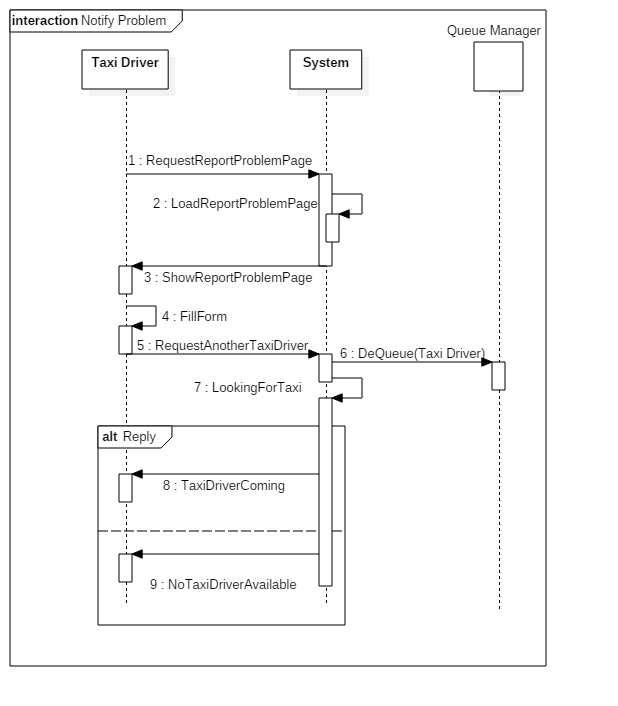
\includegraphics[width=1\textwidth,bb = 0 0 200 100, draft, type=eps]{NotifyProblem}


\subsection{Performance requirements}
\begin{itemize}
\item The system should support at least all the taxi driver registered
into the Town Database 
\item The system should elaborate user incoming information 
\item The system should provide the faster path for each ride 
\item The system should calculate the final price of the ride with a maximum
error of 10\% 
\item The system should provide to a passenger the arrival time (maximum
error 20\%) and change the path in case of traffic 
\end{itemize}

\subsection{Logical database requirements}


\subsection{Design constraints}
\begin{itemize}
\item GPS precision limitations: average 3m error 
\item Internet congestion 
\end{itemize}

\subsection{Standards compliance}


\subsection{Software system attributes}


\subsection{Reliability}


\subsection{Availability}


\subsection{Security}
\begin{itemize}
\item SSL connection over the web 
\item Username and password to identify the user and taxi driver 
\item All the Operation are logged into the system 
\item The data stored inside the secondary store are encrypted 
\item The system databases has consistency check, data integrity check 
\end{itemize}

\subsection{Maintainability}


\subsection{Portability}

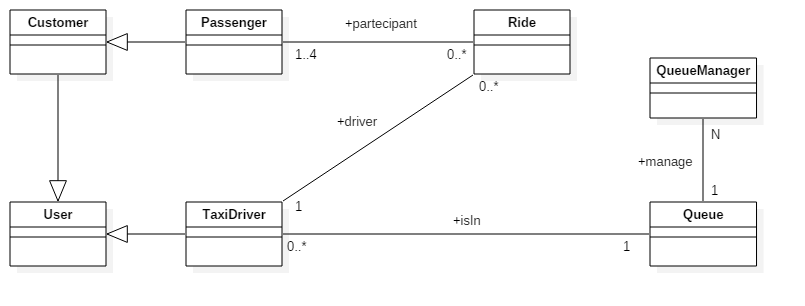
\includegraphics[width=1\textwidth,bb = 0 0 200 100, draft, type=eps]{ClassDiagram}


\subsection{Additional comments}
\end{document}
